\chapter{Quantum Relational Dynamics of JC Model
\label{chap5:RDQ_JCM_chap}}

In \refchap{chap:braun_briggs_jaynes}, we delved into the semiclassical approach to derive the Time-Dependent Schrödinger 
Equation (TDSE) governing the Jaynes-Cummings model. 
\begin{figure}[!h]
    \centering
    \includegraphics[width=0.9\textwidth, height=0.45\textheight]{chap5/JC_model.png}
    \caption{Illustration of the Jaynes-Cummings model. A two-level atom is coupled to an optical cavity (single field mode), shown on top. The energy levels of the atom that couple to the field mode within the cavity are shown in the box below.}
    \label{fig:JC_illusttration}
\end{figure}
In \refsec{sec:class_jcm_sec1}, we derived the TDSE using the position space representation by assuming a semiclassical (WKB-like) wave function for the field mode and then 
we presented a alternative derivation, in \refsec{sec:sec:class_jcm_sec2} making use of coherent representatian.
However,  both these approaches inherit the concept of ``time" as a purely classical parameter, compromising its deeper and more fundamental nature.

In contrast, in \refchap{chap:sebgem_Rel}, we presented a purely quantum framework to describe the dynamics of the general interacting system. Here, ``time" emerges as a symmetry parameter stemming from the principle of global invariance of the global energy eigenstate of the total Hamiltonian. A natural question arises: Are both of these different-looking approaches to describe the dynamics of the system equivalent? If yes, then in what limit? In this chapter, we aim to address these questions.

We start by adopting the Jaynes-Cummings Hamiltonian as our model system. We then explore the Jaynes-Cummings model from the perspective of Quantum Relational Dynamics. 
We aim to scrutinize the transition from a purely quantum system to semiclassical regimes,  as previously discussed in \refchap{chap:braun_briggs_jaynes}, and to juxtapose the dynamics as characterized by the two distinct approaches. We demonstrate that the two approaches yield identical results under appropriate limits (consistent with the semiclassical treatment in previous Chapters). 
%Interestingly, the analysis also hints at the presence of a superselection rule.

We assume our Hamiltonian to be of the form,

\begin{mdframed}
\begin{eqnarray}
        \label{eq:chap5_JCM_Hamiltonian}
        \oper{H} = \frac{\hbar \omega_0}{2} \oper{\sigma}_z + \hbar \omega \left(\oper{a}^\dagger \oper{a} + \frac{1}{2}\right) 
        + \hbar g \oper{\sigma}_x\left(\oper{a} + \oper{a}^\dagger\right). 
\end{eqnarray}
\end{mdframed}


Under dipole-approximation and rotating-wave approximation~\cite[Chap 2]{Bina_JC_tutorial} the Hamiltonian can be written as
\begin{mdframed}
\begin{equation}
        \label{eq:chap5_JCM_Hamiltonian_RWA}
        \oper{H} = \frac{\hbar \omega_0}{2} \oper{\sigma}_z + \hbar \omega \left(\oper{a}^\dagger \oper{a} + \frac{1}{2}\right) 
        + \hbar g \left(\oper{\sigma}_+ \oper{a} + \oper{\sigma}_- \oper{a}^\dagger\right).
\end{equation}
\end{mdframed}

\section[Exact Energy Eigenstate of JC-Hamiltonian]{Exact Energy Eigenstate of JC-Hamiltonian (resonant case)}

In the specific scenario of the Hamiltonian in Equation \ref{eq:chap5_JCM_Hamiltonian_RWA}, when 
\(\omega  = \omega_0\), known as the 
``resonance case," the system becomes exactly solvable.
This model is characterized by the Hamiltonian operator\footnote{Here, we dropped the \(1/2\) term from \(H_c\), 
simplifying calculations. This adjustment doesn't affect our analysis.}
\begin{equation}
        \label{eq:chap5_JCM_Hamiltonian_resonance}
        \oper{H} = \frac{\hbar\omega}{2} \oper{\sigma}_z + \hbar \omega \oper{a}^\dagger \oper{a}
        + \hbar g \left(\oper{\sigma}_+ \oper{a} + \oper{\sigma}_- \oper{a}^\dagger\right). 
\end{equation}
It portrays the resonant interaction between two energy levels of an atom and a single boson field mode.
To understand how this system evolves over time, we initially aim to compute the unitary evolution operator 
$U(t) = e^{-i t H/\hbar}$ through the diagonalization of $H$. Once we achieve an eigenvalue decomposition 
$H = \sum_n \epsilon_n \lvert \epsilon_n \rangle \langle \epsilon_n \rvert$, it follows that:

\begin{equation}
U(t) = \sum_n e^{-i t \epsilon_n/\hbar} \lvert \epsilon_n \rangle \langle \epsilon_n \rvert
\end{equation}

Finding such an eigenvalue decomposition is not trivial, particularly in this context, 
given the infinite-dimensional nature of the underlying Hilbert space. However, the 
JC-Hamiltonian possesses a notably simple structure as it is block-diagonal with respect 
to the $\ket{\pm, n}$-basis. The diagonalization of the JC-Hamiltonian in 
\refeq{eq:chap5_JCM_Hamiltonian_resonance} is given in \refapp{appen:chap5_JC_calculations} .
Once you diagonalize the Hamiltonian, the eigenvalues and eigenvectors of the JC-Hamiltonian are given by
\begin{equation}
        \label{eq:chap5_JCM_eigenvalues}
        E_{\pm, n} = \hbar \omega \left(n - \frac{1}{2}\right) \pm \hbar g \sqrt{n + 1},
\end{equation}
and the corresponding eigenvectors are
\begin{equation}
        \label{eq:chap5_JCM_eigenvectors}
        \ket*{\psi_{n,\pm}} := \frac{1}{\sqrt{2}} 
     \left( \ket*{+, n - 1} \pm \ket*{-, n} \right).
\end{equation}

We discussed the coherent state-based semiclassical approximation in Chapter 
\ref{chap:braun_briggs_jaynes}, where the final result simply involved replacing 
the field operators, i.e., \( \oper{a} \) and \( \oper{a}^\dagger \), with their 
expectation values. Following a similar approach, we could assume the semiclassical form 
of the Hamiltonian in Equation \ref{eq:chap5_JCM_Hamiltonian_resonance} as

\begin{equation}
    \label{eq:chap5_JCM_Hamiltonian_semi}
    \begin{aligned}
        \oper{H}_{\text{semi}} = \frac{\hbar\omega}{2} \oper{\sigma}_z + \hbar \omega \langle \oper{a}^\dagger \oper{a} \rangle
    + \hbar g \left( \oper{\sigma}_+ \langle \oper{a} \rangle + \oper{\sigma}_- \langle \oper{a}^\dagger \rangle \right),\\
    = \frac{\hbar\omega}{2} \oper{\sigma}_z + \hbar \omega N 
    + \hbar g \alpha\left( \oper{\sigma}_+ e^{-it\omega} + \oper{\sigma}_- e^{it\omega} \right),
    \end{aligned}
\end{equation}
where \(\langle a(t) \rangle = \alpha e^{-i\omega t}\). This leads to the evolution operator being expressed as
%\begin{align}
%        \tilde{U}(t) &= 
%                \cos(\Omega t) \left(e^{-i t \omega \frac{1}{2}}\ket{+}\bra{+} + 
%                e^{i t \omega \frac{1}{2}}\ket{-}\bra{-} \right)  \nonumber\\
%                &- i \sin(\Omega t)
%                 \left( e^{-i t \omega \frac{1}{2}}\ket{+}\bra{-}
%                + e^{i t \omega \frac{1}{2}}\ket{-}\bra{+}\right)
%\end{align}
\begin{align}
        \tilde{U}(t) &= 
                \cos(\Omega t) \left(\ket{+}\bra{+} + 
                \ket{-}\bra{-} \right)  \nonumber\\
                &- i \sin(\Omega t)
                 \left( \ket{+}\bra{-}
                +\ket{-}\bra{+}\right)
\end{align}
where \(\Omega = \frac{g\alpha}{\hbar}\). We will see in the next section that the semiclassical limit can be made more rigorous
under the limits discussed \refchap{chap:braun_briggs_jaynes}, i.e., in the limit of 
large photon number and weak ``back-coupling'' from the quantum system.

\section{Semiclassical JC-Hamiltonian  in Large Amplitude and Weak Interaction Limit\label{sec:chap5_large_amplitude_weak_g}}

The emergence of the semiclassical model occurs when fields are in
coherent states. However, recovering the semiclassical behavior is not straightforward by merely substituting coherent states (as we did in \refeq{eq:chap5_JCM_Hamiltonian_semi}). 
To elaborate, we can expect this to happen under specific conditions~\cite{semiclassical_limit_JC_PRL}:
\begin{itemize}
    \item \textbf{Large Amplitude of Coherent State}: When the amplitude of the coherent state is substantial, 
    the quantum fluctuations (i.e., the influence of atom onto the field in our model!) become less significant, 
    resembling classical behavior.
    \item \textbf{Weak Atom-Mode Coupling}: If the coupling between the atom and the mode (field) is weak, 
    the quantum effects become less pronounced, favoring semiclassical behavior.
\end{itemize}
In this section, we'll explore an interesting limit of the system. We'll consider what happens when the factor, $g = \frac{\Omega}{|\alpha|} \to 0$, as $|\alpha| \rightarrow \infty$. Here, $\Omega$ represents a fixed constant. While we won't delve into rigorous proofs, the following discussion will argue that, under these conditions, the dynamics of the atomic system can still be described by unitary evolution. To begin, let's recall the form of coherent states
%Here, we will attempt to make this idea more concrete by considering the  limit where $g = \frac{\Omega}{|\alpha|}$, and $|\alpha| \rightarrow \infty$, where $\Omega$ is a constant. In the following discussion, we will argue, albeit not in a particularly rigorous manner, that we can regain a unitary evolution on the atom in this limit. Let's first recall the form of coherent states:
\begin{equation}
    \ket{\alpha} = e^{-\frac{1}{2}|\alpha|^2} \sum_{n=0}^{\infty} \frac{\alpha^n}{\sqrt{n!}} \ket{n}
\end{equation}
    
A unique feature of these states is that the particle number has a Poisson Distribution. In other words, the probability of finding the system in photon number state, \(\ket{n}\) is given by:
\begin{equation}
    \mathrm{p}_n = \abs*{\bra*{n}\ket*{\alpha}}^2 
    = e^{-\abs*{\alpha}^2}\frac{(\abs*{\alpha}^2)^n}{n!}
\end{equation}
Our objective is to understand the evolution of the atom when it interacts with a coherent state. 
Therefore, we aim to compute the reduced density operator of the atom, which is given by:

\begin{align}
\oper{\rho}_{\text{atom}}(t) &= 
\text{Tr}_{\text{mode}} \left( U(t)[\oper{\rho} \otimes \ket{\alpha}\bra{\alpha}]U^\dagger(t) \right) \nonumber \\
 &= \sum_n e^{-\gamma} \gamma^n \frac{V_g(n)\oper{\rho} V_g^\dagger(n)}{n!},
\end{align}

where \(\gamma = \abs{\alpha}\) and\footnote{[Refer to \refapp{appen:chap5_JC_calculations} for explicit form of \(U(t)\)]}:
\begin{align}
        \label{eq:appen_JCM_V_g}
    V_g (n) &=e^{-it\omega\frac{1}{2}}  \cos(tg\sqrt{n + 1})\ket{+}\bra{+}\\
&+ e^{it\omega\frac{1}{2}} \cos(tg\sqrt{n})\ket{-}\bra{-}\\
&- ie^{-it\omega\frac{1}{2}} \sin(tg\sqrt{n + 1}) \frac{\alpha}{\sqrt{n + 1}} \ket{+}\bra{-}\\
&- ie^{-t\omega\frac{1}{2}} \sin(tg\sqrt{n}) \frac{\sqrt{n}}{\alpha} \ket{-}\bra{+}.
\end{align}
Let's discuss a few key points. Firstly, as \( x \) increases, the function 
\( \sqrt{x} \) becomes flatter (its derivative approaches zero). Secondly, .2: The plot compares the Poisson dis-
tribution for large mean values with a square
root function. As the mean increases, the Pois-
son distribution increasingly peaks and concen-
trates around the mean, while the square root
function remains nearly flat for large valu
for large values of \( |\alpha| \), the Poisson distribution is approximately 
equivalent to the normal distribution, \begin{wrapfigure}{r}{0.5\textwidth}
  \centering
  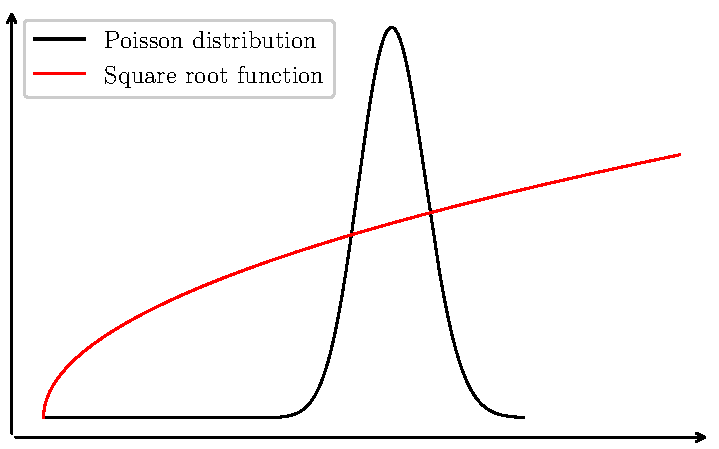
\includegraphics[width=0.48\textwidth]{figures/chap5/poisson_distribution.pdf}
  \caption{The plot compares the Poisson distribution for large mean values with a square root function. As the mean increases, the Poisson distribution increasingly peaks and concentrates around the mean, while the square root function remains nearly flat for large values. }
\end{wrapfigure}
\begin{equation}
\mathfrak{N}_{\mu, \sigma}(x) = \frac{1}{\sqrt{2\pi\sigma^2}} e^{-\frac{(x-\mu)^2}{2\sigma^2}}.
\end{equation}

In this context, the approximate normal distribution has a mean of \( |\alpha|^2 \) and a 
standard deviation of \( |\alpha| \). This implies that the distribution's width increases 
at a slower rate than the mean. Consequently, for large \( |\alpha| \), it is plausible 
that the square root remains nearly constant within the region where the Poisson/normal 
distribution is significant. Considering these observations, the subsequent reasoning 
for approximation might be easier to grasp.

\begin{equation}
\oper{\rho}_{\text{atom}}(t) = \sum_n e^{-\gamma} \gamma^n \frac{V_g(n)\oper{\rho} V_g^\dagger(n)}{n!}
\end{equation}
By approximating the weighted sum over the Poisson distribution with the integral weighted by 
the normal distribution \( \mathfrak{N}_{\mu, \sigma}(x)\), having a mean (\( \mu =  |\alpha|^2 \)) 
and standard deviation (\( \sigma = |\alpha| \)), we obtain

\begin{equation}
    \oper{\rho}_{\text{atom}}(t)\approx \int \mathfrak{N}_{\mu, \sigma}(x) V(t, x) \oper{\rho} V(t, x)^{\dagger} dx
\end{equation}
We cut away the tails of the integral at (\( s \)) standard deviations

\begin{equation}
    \oper{\rho}_{\text{atom}}(t)\approx \int_{|\alpha|^2 - s|\alpha|}^{|\alpha|^2 + s|\alpha|}\mathfrak{N}_{\mu, \sigma}(x) V(t, x) \oper{\rho} V(t, x)^{\dagger} dx
\end{equation}
Change of variables (\( x \to x|\alpha| + |\alpha|^2 \))

\begin{equation}
    \label{eq:appen_JCM_rho_atom_t}
    \begin{aligned}
        \oper{\rho}_{\text{atom}}(t)= \int_{-s}^{s} \mathfrak{N}_{0, 1}(x) V(x|\alpha| + |\alpha|^2) 
    \oper{\rho} V(x|\alpha| + |\alpha|^2)^{\dagger} dx
    \end{aligned}
\end{equation}
Now we put in our assumption that \(g = \hbar\Omega / \abs*{\alpha}\). Let's assume, 
for simplicity, that \(\alpha = \abs*{\alpha}\), i.e., it's real. Then \refeq{eq:appen_JCM_V_g} becomes
\begin{align}
    V_{\Omega/|\alpha|}(x|\alpha| + |\alpha|^2) 
    &= e^{-i t \omega \frac{1}{2}}\cos \left( t\Omega \sqrt{1 + \frac{x}{\abs*{\alpha}}+ \frac{1}{\abs*{\alpha}^2}} \right) \ket{+}\bra{+} \nonumber \\
    &+ e^{i t \omega \frac{1}{2} }\cos \left( t\Omega \sqrt{1 + \frac{x}{\abs*{\alpha}}} \right) \ket{-}\bra{-} \nonumber \\
    &- i e^{-i t \omega \frac{1}{2} }\sin \left( t\Omega \sqrt{1 + \frac{x}{\abs*{\alpha}} + \frac{1}{\abs*{\alpha}^2}} \right) \frac{1}{\sqrt{1 + \frac{x}{\abs*{\alpha}} + 1}} \ket{+}\bra{-} \nonumber \\
    &- i e^{i t \omega \frac{1}{2}} \sin \left( t\Omega \sqrt{1 + \frac{x}{\abs*{\alpha}}} \right) \sqrt{1 + \frac{x}{\abs*{\alpha}}} \ket{-}\bra{+}. \nonumber
\end{align}
Since, \(-s < x < s\), with \(s\) constant, in the limit of \(|\alpha| \to \infty\),
\begin{align}
        \label{eq:appen_JCM_V_g_limit}
    \tilde{U}(t) &:= \lim_{\abs*{\alpha}^2 \to \infty} 
    V_{\Omega/|\alpha|}(x|\alpha| + |\alpha|^2)  \nonumber \\
    &= \cos(\Omega t) \left(e^{-i t \omega \frac{1}{2}}\ket{+}\bra{+} + 
    e^{i t \omega \frac{1}{2}}\ket{-}\bra{-} \right)  \nonumber \\
    &- i \sin(\Omega t)
     \left( e^{-i t \omega \frac{1}{2}}\ket{+}\bra{-}
    + e^{i t \omega \frac{1}{2}}\ket{-}\bra{+}\right)  \nonumber \\
\end{align}
Inserting this limit back into \refeq{eq:appen_JCM_rho_atom_t}, we obtain
\begin{align}
    \oper{\rho}_{\text{atom}}(t) &\approx \int_{-s}^{s} \mathfrak{N}_{0, 1}(x) \tilde{U}(t) \oper{\rho} \tilde{U}(t)^{\dagger} dx \nonumber\\
        &\approx \tilde{U}(t) \oper{\rho} \tilde{U}(t)^{\dagger}.
\end{align}

Hence in the limit of large \(\alpha\) and weak interaction, we get the 
semiclassical limit. The final form of the evolution operator is given in \refeq{eq:appen_JCM_V_g_limit}, i.e., 

\begin{mdframed}
    \begin{align}
    \label{eq:appen_JCM_V_g_limit2}
    \tilde{U}(t) 
    &= \cos(\Omega t) \left(e^{-i t \omega \frac{1}{2}}\ket{+}\bra{+} + 
    e^{i t \omega \frac{1}{2}}\ket{-}\bra{-} \right)  \nonumber \\
    &- i \sin(\Omega t)
     \left( e^{-i t \omega \frac{1}{2}}\ket{+}\bra{-}
    + e^{i t \omega \frac{1}{2}}\ket{-}\bra{+}\right) 
\end{align}
\end{mdframed}

\section{Numerical Results: Comparing Quantum Relational Dynamics with Semiclassical Dynamics
\label{sec:chap5_numerical_results}}

\subsection*{JC-Model: Non Rotating Wave Approximation} 
\begin{figure}[!h]
    \centering
    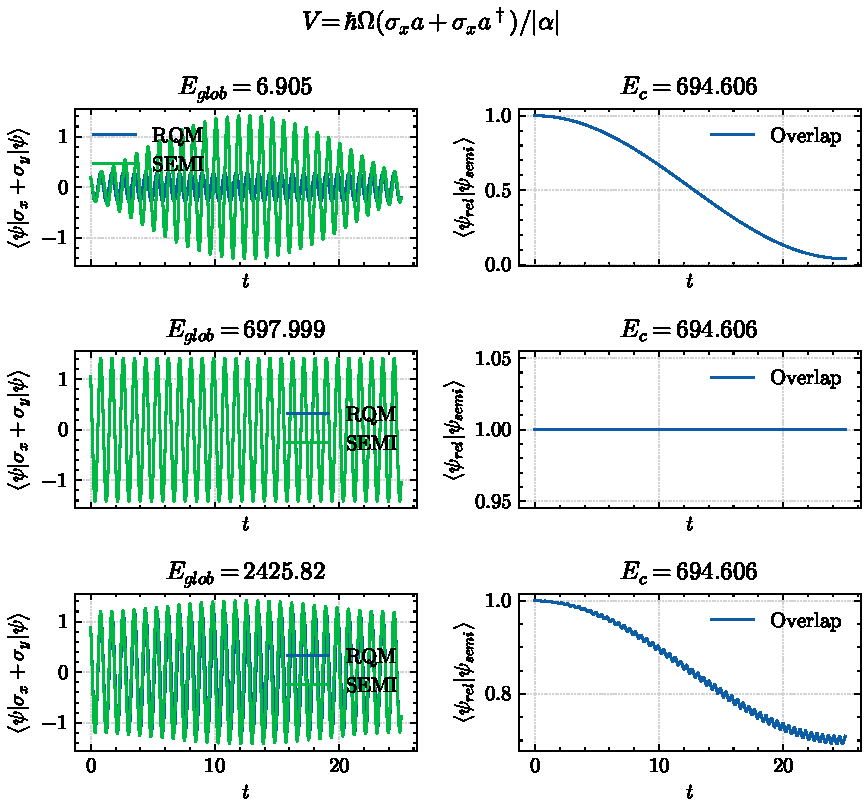
\includegraphics{chap5/semi_vs_quant_linear.pdf}
    \caption{Expectation value
        \(\bra*{\psi} \oper{\sigma}_x + \oper{\sigma}_z \ket*{\psi}\) v/s Time ($t$) for Semi-Classical and Quantum Relational Dynamics
    and \(\abs*{\braket*{\psi_{\mathrm{rel}}}{\psi_{\mathrm{semi}}}}\) v/s Time ($t$). The Global Eigenstates are calculated from 
    Hamiltonian as given in \refeq{eq:chap5_JCM_Hamiltonian_linear} and the semiclassical dynamics given by \refeq{eq:chap5_semi_classical_JC_Linear}. The parameters 
    are given in \reftab{tab:numerical_values_linear}
    }
     \label{fig:chap5_linear_semi_vs_quant}
\end{figure}


\reffig{fig:chap5_linear_semi_vs_quant} depict the expectation value of the operator  \(\oper{\sigma}_x + \oper{\sigma}_y\), 
computed using the relational evolution described by the Hamiltonian in Equation \refeq{eq:chap5_JCM_Hamiltonian}., i.e., 
\begin{eqnarray}
    \label{eq:chap5_JCM_Hamiltonian_linear}
    \oper{H} = \frac{\hbar \omega}{2} \oper{\sigma}_z + \hbar \omega \left(\oper{a}^\dagger \oper{a} + \frac{1}{2}\right) 
    + \hbar \frac{ g}{\abs*{\alpha}} \oper{\sigma}_x\left(\oper{a} + \oper{a}^\dagger\right).
\end{eqnarray}
\begin{figure}[!h]
    \centering
    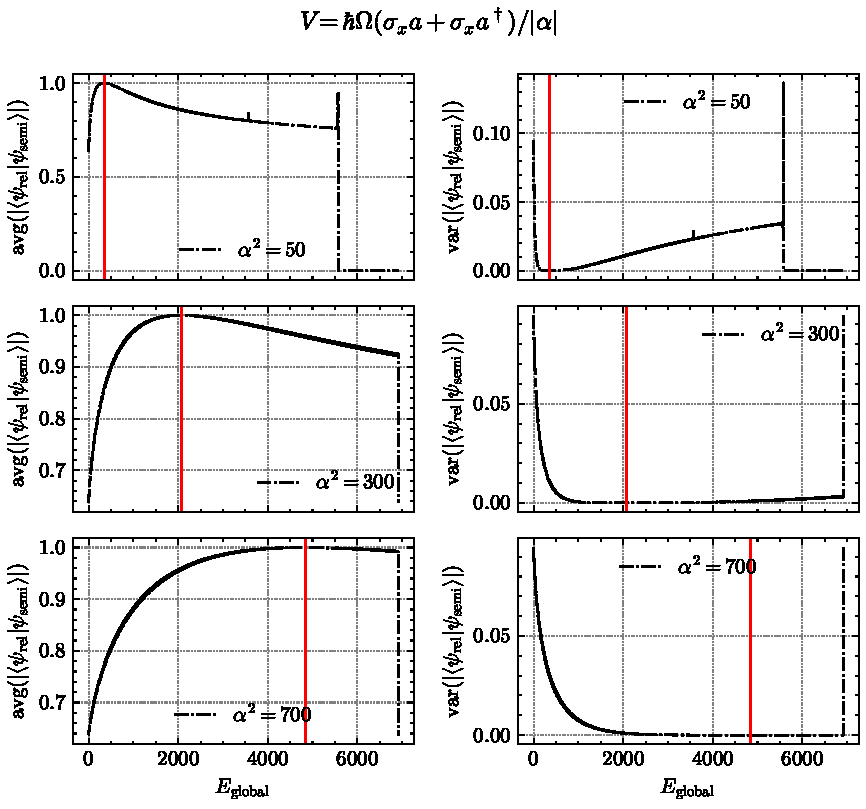
\includegraphics{chap5/overlap_average_linear.pdf}
    \caption{
     The plots shows the average $\abs*{\braket*{\psi_{rel}}{\psi_{semi}}}^2$ and 
     variance $\abs*{\braket*{\psi_{rel}}{\psi_{semi}}}^2$ over \([0, 4\pi/\omega]\) Time domain v/s corresponding global eigenenergy. The red lines represent \(E_c\).
     The Global Eigenstates are calculated from 
    Hamiltonian as given in \refeq{eq:chap5_JCM_Hamiltonian_linear} and the semiclassical dynamics given by \refeq{eq:chap5_semi_classical_JC_Linear}. The parameters 
    are given in \reftab{tab:numerical_values_linear}}
     \label{fig:chap5_linear_overlap_avg}
\end{figure}
and the the semi-classical Hamiltonain as given in \refeq{eq:class_jcm_eq30}, i.e., 
\begin{eqnarray}
\label{eq:chap5_semi_classical_JC_Linear}
    \oper{H}_{\text{semi}} = \frac{\hbar\omega}{2} \oper{\sigma}_z 
    + \hbar \frac{g}{\abs*{\alpha}} \oper{\sigma}_x\left( \alpha e^{-it\omega} + \alpha e^{it\omega} \right).
\end{eqnarray}

The clock (environment) quantum state, onto which the global eigenstate is projected 
to extract the 
quantum dynamics, 
are takes to be the
the coherent states \(\ket*{\alpha (t)}\), where \(\alpha(t) = \alpha e^{-i\omega t}\). The system's quantum state then one gets according to \refeq{eq:nonint_sys_evol}, i.e.,  
\begin{equation}
    \ket*{\psi_{rel}(t)} = \mathcal{N} \innerGlob{\alpha(t)}{\Psi_{\mathrm{glob}}},
    \mathcal{N} = \frac{1}{\sqrt{\lvert \lvert \innerGlob{\alpha(t)}{\Psi_{\mathrm{glob}}} \rvert \rvert^2}}
\end{equation}
where \(\ket*{\Psi_{E_{glob}}}\) is an eigenstate of \refeq{eq:chap5_JCM_Hamiltonian_linear}. 

The initial state is taken as \(\ket*{\psi_{semi}(0)} = N\innerGlob{\alpha(0)}{\Psi_{E_{glob}}}\), where $N$ denotes normalization, for the semiclassical time evolution and plots are shown 
for three different global energy eigenstates and a fixed \(E_c(\alpha^2) = \hbar \omega \abs*{\alpha}^2\). \reffig{fig:chap5_linear_semi_vs_quant} also shows the overlap \(\abs*{\braket*{\psi_{rel}}{\psi_{semi}}}\)
for same time evolution. \reffig{fig:chap5_linear_overlap_avg} illustrates the average and the 
variance of the absolute value of overlap \(\abs*{\braket*{\psi_{rel}}{\psi_{semi}}}\) over two time period, 
for three different values of \(E_c(\alpha^2)\) (depicted as red vertical lines in the plots). 

The parameters utilized for the numerical calculations are listed below in \reftab{tab:numerical_values_linear}.
\begin{table}[!ht]
    \centering
        \begin{tabular}{|c|c|c|c|c|}
            \hline
            Parameter & $g$ & $\omega$ & $N_{\text{cutoff}}$ & $\hbar$ \\
            \hline
            Value & $2\pi/100$ & $2.2\pi$ & $1000$ & $1$ \\
            \hline
        \end{tabular}
    \caption{Parameters used for Numerical Results in \reffig{fig:chap5_linear_overlap_avg} and 
    \reffig{fig:chap5_linear_semi_vs_quant}}
    \label{tab:numerical_values_linear}
\end{table}


%As can be seen, the plots show that the average overlap is maximized for relational states 
%where the energy eigenvalue of the global eigenket closely matches the energy of the semiclassical
%conditional state \(E_c(\alpha^2) = \hbar \omega \bra*{\alpha}\oper{a}^\dagger \oper{a}\ket*{\alpha}
%= \hbar \omega \abs*{\alpha^2}\) 



\subsection*{JC-Model: Rotating Wave Approximation}
\begin{figure}[!h]
    \centering
    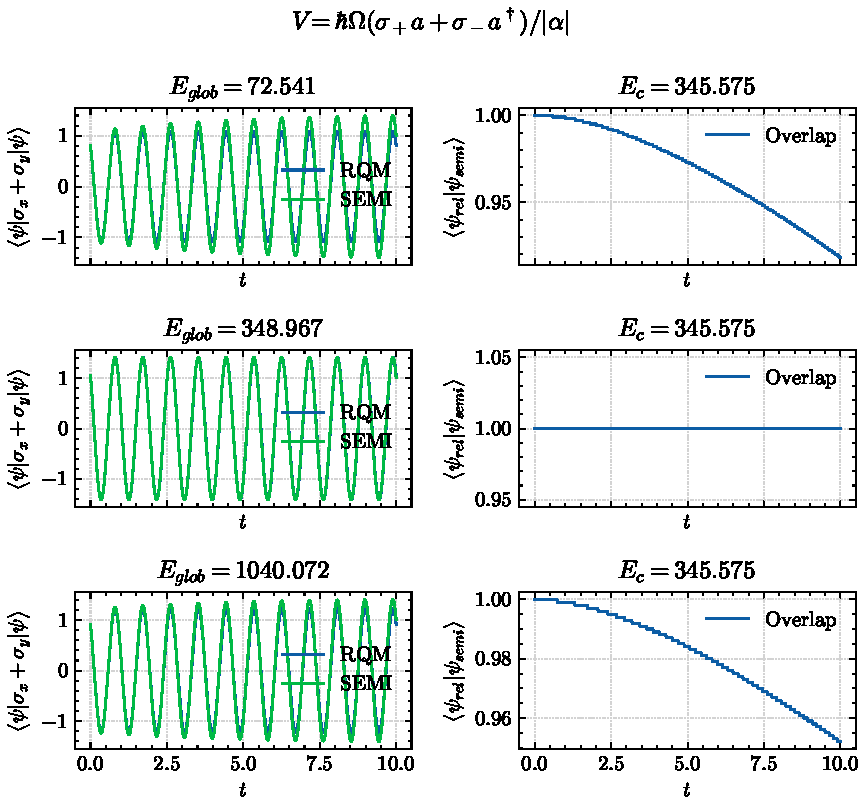
\includegraphics{chap5/semi_vs_quant_JC.pdf}
    \caption{
    Expectation value
        \(\bra*{\psi} \oper{\sigma}_x + \oper{\sigma}_z \ket*{\psi}\) v/s Time ($t$) for Semi-Classical and Quantum Relational Dynamics
    and \(\abs*{\braket*{\psi_{\mathrm{rel}}}{\psi_{\mathrm{semi}}}}\) v/s Time ($t$). The Global Eigenstates are calculated from 
    Hamiltonian as given in \refeq{eq:chap5_JC_rotwave_hamiltonian} and the semiclassical dynamics given by the unitary operator in \refeq{eq:chap5_JC_rotwave_unitary_semi}. The parameters 
    are given in \reftab{tab:numerical_values_JC}
    }
    \label{fig:chap5_JCM_semi_vs_quant}
\end{figure}


Similar to the non-rotating wave approximation, we compare the expectation values of the operator
\(\oper{\sigma}_x + \oper{\sigma}_y\) in \reffig{fig:chap5_JCM_semi_vs_quant}, as described by the Hamiltonain in \refeq{eq:chap5_JCM_Hamiltonian_resonance}, i.e., 
\begin{eqnarray}
\label{eq:chap5_JC_rotwave_hamiltonian}
    \oper{H} = \frac{\hbar \omega}{2} \oper{\sigma}_z + \hbar \omega\oper{a}^\dagger \oper{a}
    + \hbar \frac{g}{\abs*{\alpha}} \left(\oper{\sigma}_+ \oper{a} + \oper{\sigma}_- \oper{a}^\dagger\right).
\end{eqnarray}
and the semi-classical unitary evolution operator derived as in \refeq{eq:appen_JCM_V_g_limit2}, i.e.,
\begin{eqnarray}
\label{eq:chap5_JC_rotwave_unitary_semi}
    \tilde{U}(t) 
    &= \cos(\Omega t) \left(e^{-i t \frac{\omega}{2\hbar}}\ket{+}\bra{+} + 
    e^{i t \frac{\omega}{2\hbar}}\ket{-}\bra{-} \right)  \nonumber \\
    &- i \sin(\Omega t)
     \left( e^{-i t \frac{\omega}{2\hbar}}\ket{+}\bra{-}
    + e^{i t \frac{\omega}{2\hbar}}\ket{-}\bra{+}\right) 
\end{eqnarray}




Similar to the case of non-rotating wave approximation, we compute the average and the 
variance of the absolute value of overlap \(\abs*{\braket*{\psi_{rel}}{\psi_{semi}}}\) over two time period, 
for three different values of \(E_c(\alpha^2)\) (depicted as red vertical lines in the plots)
in \reffig{fig:chap5_JCM_overlap_avg}.

\begin{table}[!ht]
    \centering
        \begin{tabular}{|c|c|c|c|c|}
            \hline
            Parameter & $\Omega = g$ & $\omega$ & $N_{\text{cutoff}}$ & $\hbar$ \\
            \hline
            Value & $2\pi/100$ & $2.2\pi$ & $1000$ & $1$ \\
            \hline
        \end{tabular}
    \caption{Parameters used for Numerical Results in \reffig{fig:chap5_JCM_semi_vs_quant} and 
    \reffig{fig:chap5_JCM_overlap_avg}}
    \label{tab:numerical_values_JC}
\end{table}

\begin{figure}[!h]
    \centering
    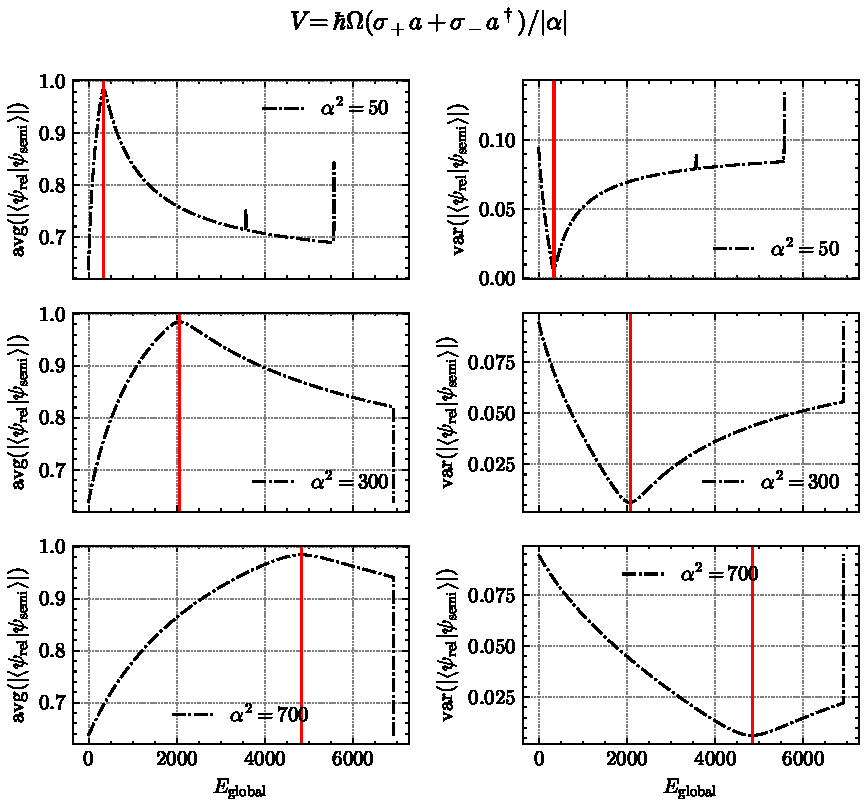
\includegraphics{chap5/overlap_average_JC.pdf}
    \caption{The plots shows the average $\abs*{\braket*{\psi_{rel}}{\psi_{semi}}}^2$ and 
     variance $\abs*{\braket*{\psi_{rel}}{\psi_{semi}}}^2$ over \([0, 4\pi/\Omega]\) Time domain v/s corresponding global eigenenergy. The red lines represent \(E_c\).
     The Global Eigenstates are calculated from 
    Hamiltonian as given in \refeq{eq:chap5_JC_rotwave_hamiltonian} and the semiclassical dynamics given by the unitary operator in \refeq{eq:chap5_JC_rotwave_unitary_semi}. The parameters 
    are given in  \reftab{tab:numerical_values_JC}}
     \label{fig:chap5_JCM_overlap_avg}
\end{figure}


\newpage 


\section{Discussion}
The numerical results presented in \refsec{sec:chap5_numerical_results} show a good agreement 
between the classical limit of the quantum relational theory and the semiclassical theories
discussed in \refchap{chap:braun_briggs_jaynes} and \refsec{sec:chap5_large_amplitude_weak_g}, under appropriate limits. 
The agreement is more pronounced for the non-rotating wave approximation than the rotating wave approximation. This is expected as the rotating wave approximation is a more stringent approximation and the
agreement is expected to be better for the non-rotating wave approximation.
The agreement is close when the \(E_c \approx E_{\mathrm{glob}}\), 
i.e., the energy carried by the environment state is near the energy of the global state. Additionally,  the above analysis reveals a key trend, as we increase the average photon number (\(\alpha^2\)) and while the energy 
of the global eigenstate
is close to the energy of the environment conditional state, the agreement between the two approaches improves (can be seen as the graphs flatten out more around the red vertical line as the average photon number increases.
it can be seen both in 
\reffig{fig:chap5_linear_overlap_avg} and \reffig{fig:chap5_JCM_overlap_avg}. 
Our numerical results align with the conditions outlined in previous chapters for a classical treatment of the environment. These conditions stipulate that the environment should possess most of the closed system's energy content and since, for our case, the coupling \(g \propto \frac{1}{\abs*{\alpha}}\). Hence, for \(\abs*{\alpha} \to \infty \implies g \to 0\). This signifies a weak interaction limit, where the ``back coupling", or the influence of the quantum system on the environment, becomes negligible.

\paragraph{Coherent states as clock states:} Our research identified coherent states as the optimal candidates for ``clock states" within the quantum relational approach. In this context, the classical limit of the quantum approach aligns seamlessly with established semiclassical theories. As discussed in~\cite{braun2004classical}, coherent states offer a significant advantage in semiclassical theory. They elegantly overcome the challenge of defining time derivatives near classical turning points, leading to a more robust treatment of the problem. 
Another intriguing aspect of coherent states is their potential connection to decoherence. Theoretical studies have conclusively demonstrated that when a single-mode boson field interacts with its environment and undergoes decoherence – the process by which quantum systems lose their superposition and entanglement properties – the field transitions naturally to a coherent state. Remarkably, the only solution of the ``master equation" that remains pure in the presence of decoherence are coherent states (gaussian states)~\cite{dutra1998decoherence, zuerk_coherent_state_1993}. 


